\chapter{Implementação da solução proposta}
\label{cap:Implementacao}

% falta falar sobre filesystem vfs e como chegar ao socket file private\_data para alem da parte de interrupts, tasklets e bottomhalfs bem como sobre os contextos de execucao
Falta falar sobre os motivos e a estrutura desejada para esta implementação

\section{MRoP e sua implementação}
\label{sec:mrop_implementation}

A implementação da solução MRoP teve em consideração vários aspectos: desenvolvimento de código minimalista, reduzida alteração do código do núcleo, utilização de \textit{APIs} internas, opaco à implementação da biblioteca \textit{PCap}, de forma a poder ser integrada nesta.
A implementação autocontida em um módulo, de modo a poder ser carregado e libertado do núcleo pelo administrador.
Modulariazação das diversas componentes, permitindo assim um desenvolvimento de cada subcomponente de forma autónoma.

No capítulo \ref{} foram apresentados alguns sistemas que permitem efectuar monitorização ou filtragem de pacotes com indicação de um processo.
No MRoP, apesar de utilizar o sistema de instrumentação do núcleo \textit{KProbes}, diferencia-se das soluções apresentadas, sendo totalmente implementado dentro do núcleo, com uma reduzida utilização de memória e uma reduzida perturbação do sistema.

Como apresentado na secção \ref{}, o sistema de monitorização de rede é utilizado para cada pacote que entra ou saí do sistema.

\begin{figure}[ht]
\centering
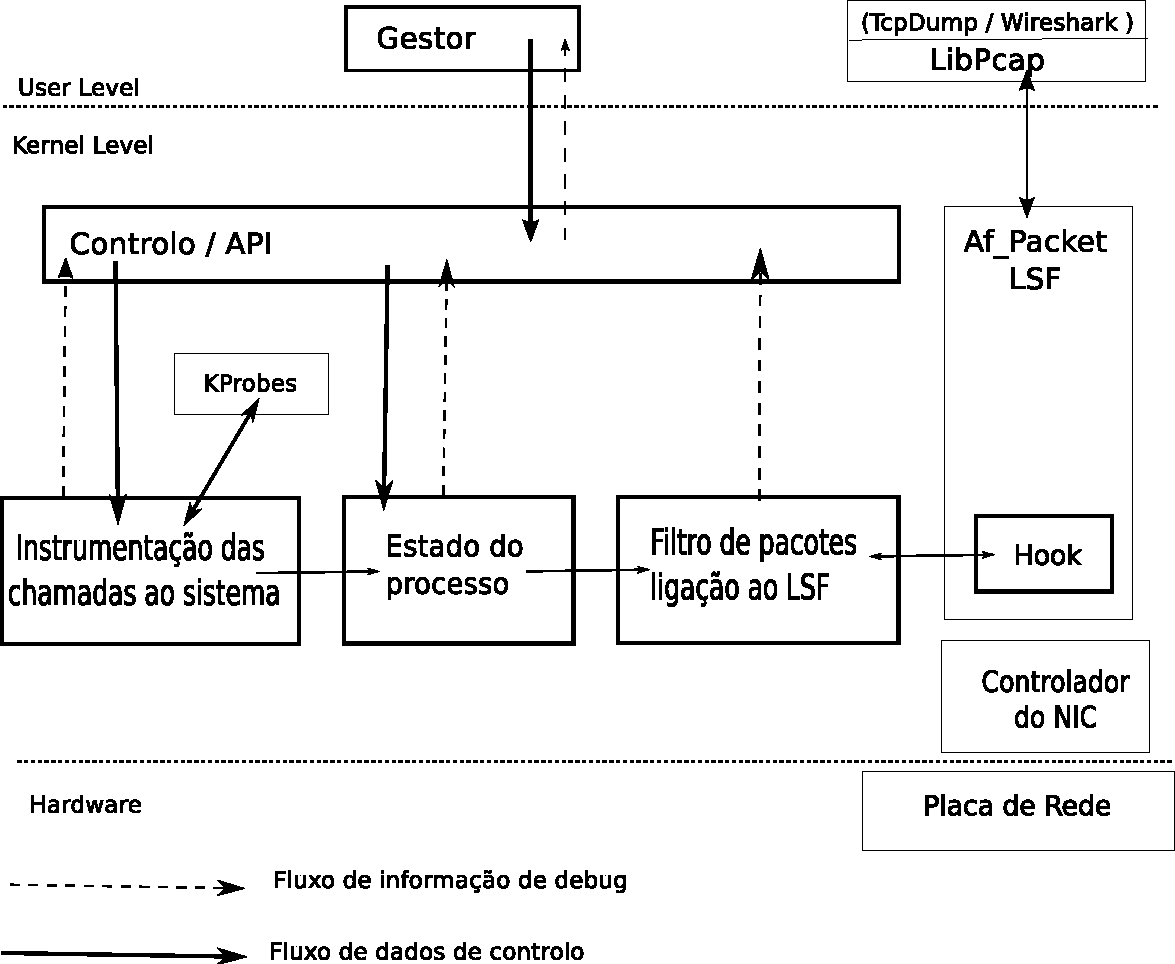
\includegraphics[scale=0.5]{arquitectura.pdf}
\caption{Arquitectura geral}
\label{fig:general_architecture}
\end{figure}





Por cada pacote ter de atravessar toda a arquitectura de rede incluida no \textit{vfs} seria demasiado pesado para o sistema.

------- apresentar as diversas seccoes ao leitor ----------------

Nas subsecções seguintes irão ser apresentados os 4 subcomponentes do MRoP.


\section{Estado dos \textit{sockets}}

De forma a manter a informação sobre os endereços e portos que uma aplicação está a utilizar, sem que seja necessário consultar os sockets que esta está a utilizar, foi necessário criar um repositório de dados onde estivesse a informação relevante para as decisões do filtro de captura.

As abordagens para a criação de um repositório de dados com base nas estruturas de dados:

Necessidades de inserção, remoção e consulta. Qualquer uma destas operações deverá ser efectuada com celeridade procurando estruturas que tenham uma complexidade temporal BigO O(1) ou O(log n).

\subsection{Com suporte no núcleo}
%outro titulo alternativas disponíveis

\begin{description}

\item[BitMap]
%\subsubsection{Bitmap}

A utilização de um mapa de bits permitiria de uma modo bastante rápido e com uma reduzida utilização de memória, saber se um determinado porto estaria em utilização por um determinado processo.
O núcleo tem suporte para tratamento de mapas de bits, ou seja, verifica se um determinado bit em um conjunto de memória está activo ou não, permitindo também afectar um determinado bit em um conjunto de memória.
Este processo apesar de extremamente rápido, carece de modularidade na utilização de multiplos endereços de rede, pois apenas controlam-se os portos, não tendo suporte para protocolos ou multiplos endereços de rede.
 
Uma solução seria agrupar os diferentes mapas de bits sob a terminologia de um endereço, mas e se fosse udp ou tcp ?
E quando um processo efectua um bind sob todas as interfaces do sistema ? 
E quando é utilizada mais uma interface virtual sob uma real ? .....


\item[Listas]





%\subsubsection{Listas duplamente ligadas}
%\subsubsection{Árvores}

\item[Árvores]
Apesar de não ser necessário percorrer os elementos ou obter os indíces de forma ordenada. 

%\paragraph{Árvore Binária}

\item[Árvore Binária]

%\paragraph{Arvores Balanceadas}
\item[Árvore Balanceada]
\textit{Red-black Tree} implementada no núcleo de operação permite efectuar

Complexidade de inserção, pesquisa e remoção é O(log n), sendo n o número de elementos da árvore.

Pode existir uma penalização no desempenho, devido à necessidade de balancear a àrvore.
Os ganhos provenientes deste balanceamento, face às àrvores não balanceadas, permite manter a complexidade média de acesso aos dados em O(log(n)), ao invés de um possível decremento até O(n), ou seja a árvore degenerar em uma lista.
\end{description}

\subsection{Sem Suporte no núcleo}

\begin{description}
%\subsubsection{Tabela de dispersão}
\item[Tabela de Dispersão]
Não existe nenhuma implementação 

%\subsubsection{Bloom Filter}
\item[Bloom Filter]
bloom filters ...

\end{description}
\paragraph*{}
A estrutura de dados escolhida para a criação do repositório de dados da componente Estado dos \textit{sockets} foi a \textit{Red-black tree}.
 Esta escolha foi principalmente à performance e à existência da implementação da estrutura no núcleo do \textit{Linux}.
 Devido a esta estrutura estar presente no núcleo do \textit{linux} permitiu que a implementação da ferramenta tivesse um ciclo de implementação mais rápido devido à confiança na ``validação`` desta estrutura pelos responsáveis do núcleo do \textit{linux}.
 
\subsection{Estrutura utilizada}
\label{sub:repo_structure}

O repositório criado através de uma árvore \textit{Red and Black} contém elementos com uma estrutura bem definida.
Esta estrutura tem de ter pelo menos um elemento, um \textit{rb\_node}, para que seja possível manipular a árvore, um elemento para comparar que serve de chave.
A estrutura anteriormente descrita contém outros elementos para além daqueles indicados, que serão descritos em seguida.

\begin{figure}[ht]
\begin{minipage}[b]{0.5\linewidth}
\centering
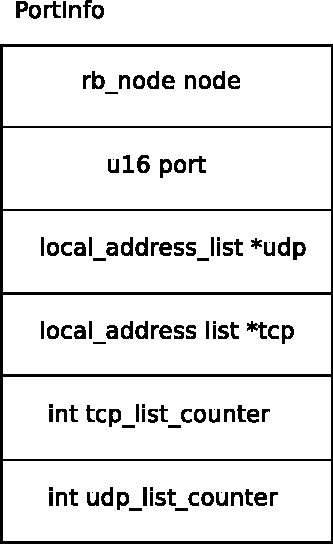
\includegraphics[scale=0.5]{portInfo_structure.pdf}
\caption{Elemento da árvore}
\label{fig:portInfo}
\end{minipage}
\hspace{0.5cm}
\begin{minipage}[b]{0.5\linewidth}
\centering

\includegraphics[scale=0.5]{local_address_list}
\caption{Lista de endereços}
\label{fig:local_address_list}
\end{minipage}
\end{figure}

Na figura \ref{fig:portInfo} está apresentada a disposição dos elementos da estrutura que \textit{portInfo}, sendo que a lista de endereços \textit{IP} das interfaces de rede são adicionados através da estrutura apresentada na figura \ref{fig:local_address_list}.
Os elementos do repositório, são instâncias da estrutura \textit{PortInfo}, adicionados através dos \textit{handlers} das funções instrumentadas.


\begin{figure}[ht]
\centering
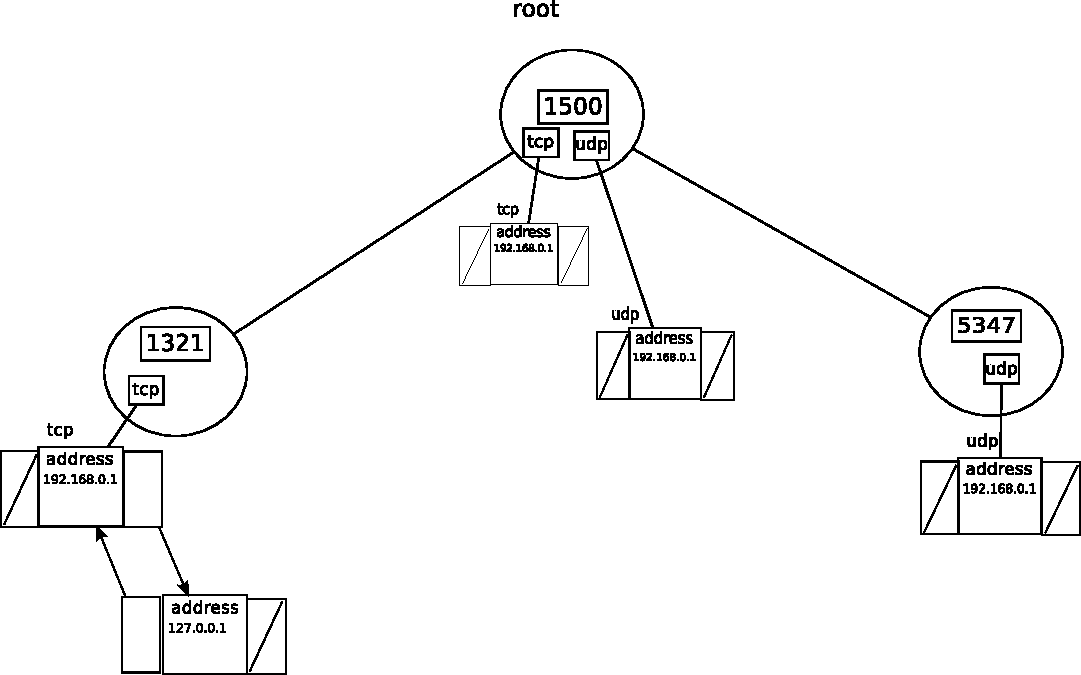
\includegraphics[scale=0.7]{repositorio_exemplo.pdf}
\caption{exemplo}
\label{fig:repo_example}
\end{figure}

\subsection{\textit{API} de comunicação interna do MRoP}
\label{sub:repo_api}

Foi criada uma \textit{API} interna ao MRoP, para permitir efectuar a inserção, consulta e remoção dos dados do repositório.
A utilização desta \textit{API} permite efectuar uma validação dos parâmetros passados às funções do repositório de dados.
Foi possível separar as componentes do MRoP através desta \textit{API}, melhorando assim a modularidade do código.

\begin{figure}[ht]
\centering
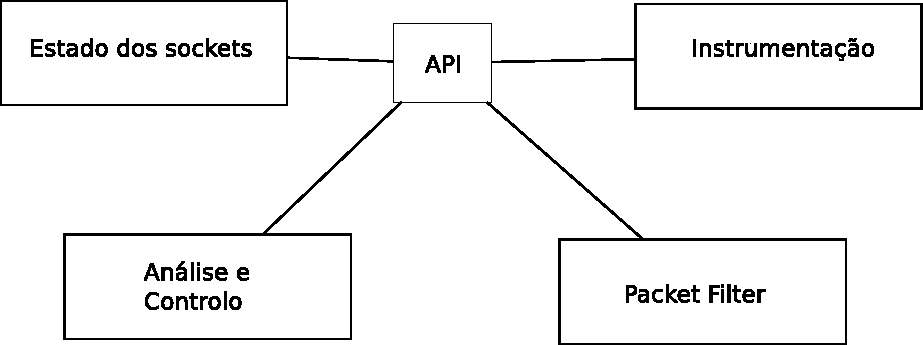
\includegraphics[scale=0.7]{API_connect_drawing.pdf}
\caption{API interna}
\label{fig:api_connect}
\end{figure}

Esta \textit{API} permite aos \textit{handlers}, das funções instrumentadas, efectuar as operações de inserção e remoção sobre a componente \textit{Estado dos sockets}.
A operação de consulta é principalmente importante para a filtragem de pacotes das interfaces de rede.

Apesar de reduzir o desempenho, porque necessita de chamar os métodos especificos ao repositório, permite que outros repositórios possam ser adicionados, permitindo modificar facilmente o código.

Apesar dos processos monitorizados terem um elevado dinamismo nas comunicações, a maior percentagem de operações sobre o reposiório serão de consultas.
As restantes operações de inserção e remoção irão ter uma percentagem igual entre elas.
É esperado que para cada inserção exista uma remoção.
Após a monitorização de um processo é esperado que a componente \textit{Estado dos Sockets}, esteja com o mesmo número de elementos, que antecedeu a monitorização.

\section{Instrumentação de funções do núcleo}

----------------------------------------------------------------------------------------------------------

Como foi anteriormente descrito em \ref{subsection:network} sobre as chamadas aos sistema para utilizar as funcionalidades de rede

Foi necessário conhecer a \textit{ABI}\ref{ABI}\cite{ABI} referente às arquitecturas suportadas, \textit{x86} e \textit{x86\_64}, para a passagem de parâmetros das chamadas aos sistema.

O sistema de \textit{KProbes} permite consultar os registos do processador onde foi efectuada a chamada à função (neste caso a chamada ao sistema).
 Por isso foram definidos 6 \textit{KRetProbes} referentes às chamadas \textit{connect}, \textit{bind}, \textit{accept}, \textit{sendto}, \textit{recvfrom} e
\textit{close}.
 Para esta última \textit{close} devido à elevada utilização desta chamada ao sistema por diferentes aplicações no sistema, foi utilizada a função \textit{qqq coisa ...  ????}

Para efectuar a monitorização das interacções de rede de um processo foi necessário recorrer à instrumentação de funções do núcleo.

Através da instrumentação de funções do núcleo foi possível manter o contexto da execução do processo.

Como apresentado e concluído na secção \ref{}, o sistema de monitorização que melhor se adequa ao problema exposto é o \textit{KProbes}.
 Deste sistema utilizou-se o \textit{KRetProbe}, de forma a instrumentar a entrada e retorno de funções.
 Obter os parâmetros de entrada das funções, principalmente o \textit{file descriptor}, tornou-se essencial.
 Para garantir que o repositório do estado do processo está coerente com o estado do núcleo, foi necessário obter o valor de retorno das funções.
 Por estas razões e porque as chamadas ao sistema têm ciclos de modificação da bastante lentos, o que evidência elevada estabilidade e consistência do núcleo, e por ser ponto de entrada do processo no núcleo foram as funções instrumentadas.

As subsecções \ref{} .... \ref{} apresentam as funções do núcleo que foram instrumentadas.

%
% faltam as subsecoes ... 
%

----------------------------------------------------------------------------------------------------------

A metodologia aplicada à resolução deste problema de desempenho, teve como base o desenvolvimento de uma componente que efectue uma análise aos canais, de comunicação de rede (\textit{sockets}) utilizados por um processo, inserir a informação necessária num repositório, e quando o pacote chegar ao sistema de monitorização utilizar o repositório para capturar ou não o pacote.

Dos diferentes sistemas analisados na secção \ref{}, aquele que sendo dinamico permitia ter uma menor sobrecarga, foi o \textit{KProbes}.
Os outros sistemas tinham componentes de \textit{logging}, que para a realização deste trabalho, teria uma sobrecarga desnecessária, afectando negativamente o desempenho.

Para além de se ter tido em consideração o sistema de instrumentação utilizado, foi também tido em consideração o número de funções a instrumentar.
A sobrecarga total exercida por esta componente é também em função do número de funções que são instrumentadas, bem como do número de vezes que estas funções são executadas.

A análise efectuada no capítulo \ref{cap:Estrutura} sobre a \textit{Arquitectura de rede em Linux}, permitiu obter uma melhor análise deste.

O MRoP, instrumenta um reduzido número de funções do núcleo pertencentes ao subsistema de rede do \textit{Linux}.
Este novo sistema foi criado monitorizar a utilização de canais da familia \textit{inet} para comunicação, tendo como particularidade a utilização de canais baseados nos protocolos \textit{tcp} e \textit{udp}.


Estes dois protocolos têm em comum algumas funções com outros protocolos de outras familias, principalmente quando as funções são as chamadas ao sistema.
De forma a dimínuir o número de funções a instrumentar, decidiu-se instrumentar as chamadas ao sistema, obtendo assim um maior nível de abstração mas também um controlo directo com o efectuado nos processos.
As chamadas ao sistema instrumentadas foram: \textit{sendto}, \textit{recvfrom}, \textit{connect}, \textit{bind}, \textit{accept} e \textit{close}.
As primeiras análises efectuadas demonstraram que apenas a chamada ao sistema \textit{close}, era executada demasiadas vezes, dimínuindo assim o desempenho global do sistema.
Esta situação é facilmente explicável, pois a chamada ao sistema \textit{close}, é utilizada extensivamente para fechar canais, sejam eles ficheiros, \textit{sockets}, \textit{pipes}, etc.
Por esta razão foi necessário encontrar a função que lida com o fecho de \textit{sockets}, permitindo desta forma reduzir a sobrecarga imposta pela instrumentação.


\subsection{Filtro de processos}
------------------------------------------------------------------------------------------------

A filtragem dos processos que efectuam as chamadas ao sistema de rede impôs um novo desafio.
 Se apenas filtrar as chamadas de um processo/pid seria apenas verificar se o pid é igual ao que se pretende é trivial e com baixa sobrecarga.
 Para um utilizador que queria analisar um processo, e não saiba qual dos fluxos do processo é responsável pela comunicação de rede, tornou-se complicado.

Com esta abordagem ainda existe a possibilidade de não se obter todas as \textit{task} do processo, caso este tenha um àrvore com mais de 3 níveis, mas a sobrecarga sobre o sistema é inferior à situação de monitorização da criação de processos no sistema.
 Estes três identificadores foram escolhidos pois permitem identificar até 3 níveis da árvore de um processo.

Seria bom colocar uma imagem de uma àrvore de processo .... 

Os identificadores têm de ser escritos para os ficheiros respectivos no \textit{DebugFs}, que serão explicados na secção \ref{}.

-----------------------------------------------------------------------------------------------------

O \textit{KProbes} é um sistema de instrumentação do núcleo, que não efectua distinção entre que funções, não inline, está a efectuar a instrumentação.
Não existindo suporte no \textit{KProbes} para filtrar o processo que está a efectuar uma chamada ao sistema, foi necessário desenvolver uma metodologia que permitisse reduzir a sobrecarga desnecessária, quando a monitorizaçãoe efectuada sobre um processo que não o desejado.

Os pontos principais continuariam a ser reduzida sobrecarga e actualização permanente do(s) processo(s) a monitorizar.
Tendo estas caracteristicas como base algumas possíbilidades foram tidas em consideração, onde o principal desafio foi conseguir manter a informação actualizada.

Uma das possíbilidades foi a criação de um repositório com a informação sobre os identificadores dos processos a monitorizar, sendo necessário novamente uma estrutura de suporte a este repositório bem como funcionalidades de adição, remoção, actualização e consulta.
Este repositório teria de conter a estrutura genológica do processo a monitorizar, bem como um componente que actualize esta informação.
A actualização desta estrutura poderia ser efectuada através da instrumentação da chamada ao sistema \textit{fork} ou \textit{clone}.
Para cada vez que fossem invocadas as funções, anteriormente mencionadas, seria efectuado uma consulta ao repositório e apartir da informação obtida neste seria ou não actualizado o repositório.
Esta possibilidade, ao contemplar a remoção de dados do repositório, necessitaria também de instrumentar a função de termino de processos.
A actualização dinamica deste repositório, sem alterar código no núcleo, necessitaria de instrumentar algumas funções no núcleo o que iria afectar o desempenho do sistema não sua totalidade, pois a criação e destruição de processos pode ser elevada.

Em alternativa, efectuou-se uma análise aos campos da estrutura que descreve um processo, a \textit{task\_struct}, de forma a compreender que forma estes dados se relacionam com os identificadores dos membros da àrvore genelógica do processo.
Desta análise obteve-se que, os identificadores \textit{pid}, \textit{tid} e \textit{ppid} permitem na grande maioria das aplicações, identificar toda a àrvore geneológica.


\subsubsection{Identificadores}

No núcleo do \textit{Linux} quando um processo é criado os identificadores \textit{pid} e \textit{tgid} são iguais.
Os processos quando efectuam

\section{Filtro de pacotes, extensão ao LSF}

No sistema de monitorização de rede um dos componentes é uma função que serve de máquina virtual às instruções do \textit{LSF}.
Esta função itera sobre o filtro executando instrução a instrução, sobre o pacote (recebido ou enviado), até encontrar uma instrução de return (\textit{BPF\_RET} ou \textit{BPF\_RET\_A}).
Consoante o valor de retorno nestas instruções o pacote analisado é ou não capturado.
Se for capturado, é efectuada uma cópia do pacote e colocado em um \textit{ring buffer} partilhado com a aplicação monitora de rede, em nível utilizador.
Caso não seja para captura a computação sobre esse pacote termina, reduzindo assim a sobrecarga da monitorização.
Por esta razão um filtro que consiga identificar rapidamente a rejeição de um pacote, permite diminuir consideravelmente a sobrecarga imposta no sistema pela monitorização.

Possivelmente o sistema de instrumentação do núcleo, \textit{KProbes} , poderia ser utilizado para invocar o novo sistema de filtragem criado e modificar o valor de retorno, caso se verifique essa necessidade.
Devido ao elevado número de vezes que a função de filtragem é invocada (uma para cada pacote, recebido ou enviado), a sobrecarga da utilização do \textit{KProbes} seria inaceitável.
Por esta razão, a única alteração efectuada ao código do \textit{Linux}, foi na função \textit{sk\_run\_filter} e a definição de um \textit{hook} para activação e desactivação deste novo sistema, ambos definidos no do ficheiro \textit{filter.c}.
Esta alteração permitiu adicionar uma nova funcionalidade à custa de uma sobrecarga muito reduzida, no sistema de monitorização, mesmo quando não estando activa a funcionalidade.
Quando monitorização de rede está activa, sem a componente MRoP, a sobrecarga introduzida é apenas a verificação se o \textit{hook} está activo ou não.

\begin{figure}[ht]
\centering
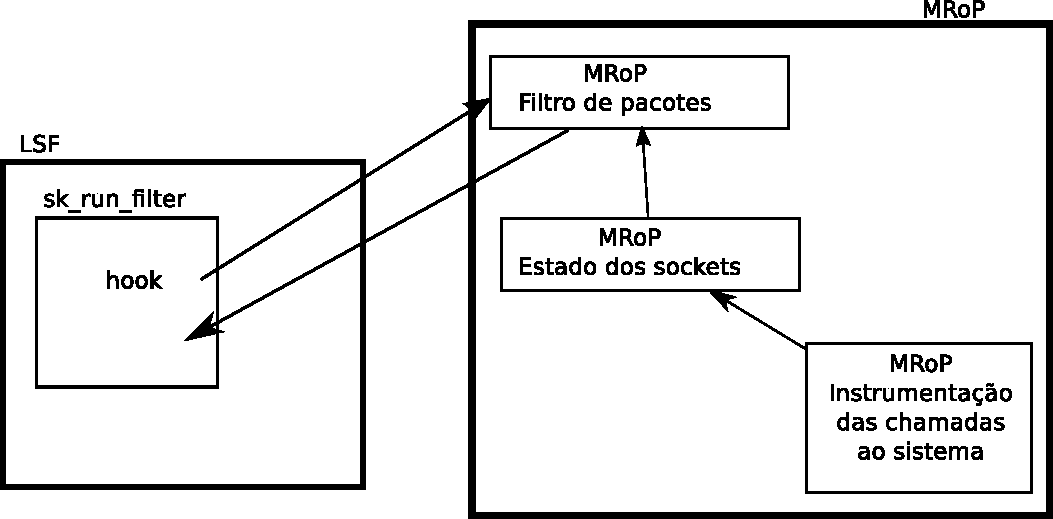
\includegraphics[scale=0.7]{run_filter.pdf}
\caption{Execução de filtragem de pacotes}
\label{fig:run_filter}
\end{figure}


\section{Informação de análise e controlo}

Devido à necessidade de obter algumas informações sobre o estado da computação dos diversos componentes da ferramenta foram criados alguns ficheiros no
sistema de ficheiros virtual \textit{DebugFs}.

Na verdade não foi só para obter o estado da computação foi também uma forma invocar o inicio da monitorização.
 Isto é, através dos ficheiros \textit{pid}, \textit{ppid}, \textit{tgid} e \textit{option}. 

\subsection{Informação do processo}


O MRoP foi desenhado para ser práticamente autónomo, apenas necessitando de configuração de alguns parâmetros essenciais ao seu funcionamento.
A componente \textit{Informação de análise e controlo}, permite efectuar o controlo sobre aspectos da instrumentação e do repositório.
A informação de análise é apenas adicionada, se o suporte para análise for activado na compilação, permitindo assim obter métricas sobre os diferentes componentes internos do MRoP.

O sistema de comunicação, entre o nível utilizador e o núcleo, utilizado foi o \textit{DebugFs}, anteriormente analisado em \ref{}.



%Quando o módulo da ferramenta é executado os indicadores de \textit{pid}, \textit{ppid} e \textit{tgid} são inicializados com o valor -1.

%Esta ferramenta de monitorização só irá passar a analisar os dados das chamadas ao sistema quando estes valores estiverem definidos e identificarem o processo que efectuou a chamada.

%\subsubsection{Sistema de Ficheiros}

%Dentro do sistema de ficheiros onde os \textit{sockets} estão incorporados, como apenas estamos interessados em analisar os sockets construidos para a familia \textit{AF\_INET} todos os sockets que não pertencerem a esta familia e não forem do tipo \textit{TCP} ou \textit{UDP} não serão mais analisados.
% Os \textit{sockets} que pertencem é então inicializado uma estrutura do tipo \textit{não me lembro ??? ver código} onde estão definidos o porto, o endereço e se são do tipo \textit{UDP} ou \textit{TCP}.

%Dependendo da chamada ao sistema realizada entre a função definida na entrada e a definida no retorno do \textit{KRetProbe}, são passados parâmetros que irão ser utilizados na função de retorno.


%\subsection{DebugFs}
%Criação de alguns ficheiros no sistema virtual \textit{configFs} para poder observar o comportamento da monitorização e dos pacotes que chegaram ao sistema de filtragem.
%A forte restrição de apenas um valor por ficheiro do \textit{SysFs} obriga a que para obter diferentes valores do sistema tenha de abrir diferentes ficheiros.
% Como o sistema de ficheiros \textit{proc} se sitia principalmente para os processos seria um bom candidado para a colocação de informação sobre 


%\section{Dificuldades}
% As chamadas ao sistema para o protocolo \textit{UDP} podem ser dificeis de analisar pois apesar de para o \textit{sendto} poder user utilizada a mesma técnica que foi utilizada para o \textit{connect}, para o \textit{recvfrom} pode ser mais dificil pois pode receber pacotes de multiplas fontes

\section{Conclusão}
\label{sec:implement_conclusion}
